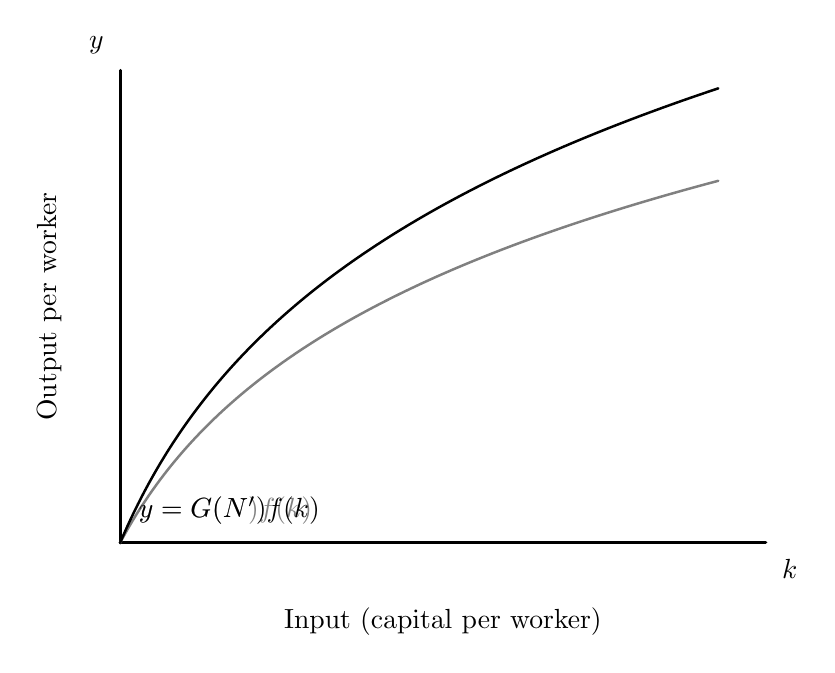
\begin{tikzpicture}[line cap=round]
  % Canvas limits
  \def\xmax{8.2}
  \def\ymax{6.0}

  % Axes
  \draw[line width=1.1pt] (0,0) -- (\xmax,0) node[below right=2pt] {$k$};
  \draw[line width=1.1pt] (0,0) -- (0,\ymax) node[above left=2pt] {$y$};

  % Axis captions
  \node[below] at (0.5*\xmax,-0.7) {Input (capital per worker)};
  \node[rotate=90] at (-0.9,0.5*\ymax) {Output per worker};

  % Base production function shape: concave, increasing
  % f(k) ∝ ln(1 + a k). Two vertical scalings represent G(N) and G(N').
  \def\a{0.8}
  \def\gLow{2.35}
  \def\gHigh{2.95}

  % Lower curve: y = G(N) f(k)
  \draw[domain=0:7.6, samples=200, smooth, gray, line width=0.9pt]
    plot(\x, {\gLow*ln(1+\a*\x)})
    node[pos=0.94, above right=3pt] {$y=G(N)f(k)$};

  % Upper curve: y = G(N') f(k)
  \draw[domain=0:7.6, samples=200, smooth, line width=0.9pt]
    plot(\x, {\gHigh*ln(1+\a*\x)})
    node[pos=0.94, above right=3pt] {$y=G(N')f(k)$};
\end{tikzpicture}